\section{Electorchemistry - mass spectrometry}\label{sec:ECMS}

Mass spectrometry is one of the most versatile and widely used analysis tools in science\cite{Gross2007, Harris2010}. It also has rich and fascinating history\cite{Griffiths2008}, some notable points in which are summarized in Figure \ref{fig:MS_timeline}. In essence, mass spectrometry is the study and use of methods to separate charged particles in high vacuum by their mass-to-charge (m/z) ratio. The mass-to-charge ratio of  all molecular and atomic ions (at non-relativistic energies) is very close to an integer multiple of one atomic mass unit per fundamental charge, and so the m/z ratio is usually stated simply as an integer with the implied units of [atomic mass unit per fundamental charge]. Some mass spectrometers have such high resolution that they can separate ions with the same nominal (integer) m/z ratio\cite{Gross2007}, but for the quadrupole mass spectrometers used in this PhD thesis, m/z is in effect an integer.

\begin{figure}[h!]
	\centering
	
\includegraphics[height=0.8\textheight]{02_Tools/fig/MS_timeline.png}
	\caption{Brief history of mass spectrometry. Most events are described in ref. \citen{Griffiths2008} and at \url{https://en.wikipedia.org/wiki/History_of_mass_spectrometry}. Several later events focus on the coupling of electrochemistry and mass spectrometry: [A], ref. \citen{Hoch1963}; [B], ref. \citen{Bruckenstein1971}; [C], ref. \citen{Wolter1984}; [D], ref. \citen{Wonders2006}; [E], ref. \citen{Henriksen2009}; [F], ref. \citen{Trimarco2015}: [G], Paper \ref{Trimarco2018}.}
	\label{fig:MS_timeline}
\end{figure}

The early development of mass spectrometry was inseparable from the fundamental study of how charged matter behaves under electric and magnetic fields in vacuum, and thus closely tied to many fundamental discoveries in early physics. This includes the discovery of the electron, the discovery of relativistic effects, and the discovery of isotopes. Mass spectrometry has been put to use in an astounding number of applications, including a prominent unsavory one: a modified mass spectrometer was used in one of the purification steps of \ch{^{235}U} for the first atomic bombs (diffusion-based methods and centrifugation have since become much more practical methods of separating this isotope)\cite{Hewlett1962}. Other applications include, for example, trace element analysis (ICP-MS) and protein sequencing (MALDI-TOF).

\begin{figure}[h!]
	
\includegraphics[width=\textwidth]{02_Tools/fig/MS_diagrams.png}
	\caption{Diagram of the components of a quadrupole mass spectrometer (QMS): \textbf{(a)}, electron impact ionization; \textbf{(b)} quadrupole mass separation; and \textbf{(c)},  secondary electron multiplier detection. Adapted from J. Gross, ``Mass Spectrometry'', ref. \citen{Gross2007}. Figure numbers in the image refer to that textbook.}
	\label{fig:MS}
\end{figure}

A mass spectrometer consists of at least three components in a vacuum vacuum chamber\cite{Gross2007}: 

\begin{enumerate}
	\item \textbf{Ion source.} The ion source for the electrochemistry-mass spectrometry (EC-MS) setups described in this Thesis is electron impact ionization (EI, Figure \ref{fig:MS}a). An electron beam is generated by heating up a filament until the high-energy tail of the Fermi distribution of the electrons in the material exceeds the work function of the material. This expels electrons into the vacuum. These electrons are accelerated through a voltage $V$ and pick up an \textit{ionization energy} of $q_\text{e}V$. The ionization energy in this diagram, and throughout this Thesis, is 70 eV. The electrons encounter the molecules to be analyzed (we'll get back to how these molecules got there) in an \textit{ion volume} and impact some of them, imparting a large energy. Many of these impact events result in the expulsion of another electron (or multiple electrons), generating a positively charged ion. Many also result in \textit{fragmentation}, or breaking of the molecules' bonds. It is these \textit{fragments} which are separated and detected by m/z ratio. First they are accelerated from the ion volume to the mass separator.
	
	\item \textbf{Mass separation.} For the EC-MS setups, this is accomplished by a quadrupole (Figure \ref{fig:MS}b). A quadrupole consists of four parallel rods separated by a distance on the order of a centimeter. The rods are connected in two pairs, which are biased by a constant DC bias superimposed on a radio-frequency AC bias. The result is that ions of a specific m/z ratio, which is a function of these two biases, are driven in a stable circular trajectory between the rods and in the plane perpendicular to the rods, whereas ions of other m/z ratios are thrown out by either the AC bias (small ions) or the DC bias (large ions). Ionized fragments enter the four rods with a velocity parallel to the rods, and those with the right m/z ratio fly in neat spirals long enough to make it through. The biases can be changed quickly to scan through a range of m/z ratios (for a \textit{mass spectrum}) or jump between specific m/z ratios of interest to monitor their signals as a function of time (for a \textit{mass-time} measurement). The separation power increases with the length of the quadrupole, and 10 cm is a typical length. 
	
	\item \textbf{Detection.} The ion fragments that make it through the quadrupole hit a detector. In the simplest case, called a \textit{Faraday cup} the detector is just a grounded piece of metal, and the current from the ground, which is equal to the current due to the ions hitting the detector, is measured. However, for higher sensitivity, with a \textit{secondary electron multiplier} (SEM), the ions hit the first of a series of charged plates, starting an electron cascade. The current coming out of the last plate, which is orders of magnitude larger than than the ion current hitting the first plate, is recorded as the \textit{mass spectrometer signal}. For the EC-MS setups in this Thesis, we use a SEM.
\end{enumerate}

Each of the three components above necessarily operate in high vacuum\cite{Gross2007, PfeifferKnowhow}. 
%(1): The mean free path of electrons should be greater than the distance from the filament to the center of the ion volume, generally a few centimeters,  necessitating a vacuum better than $\sim 10^{-4}$ mbar\cite{Concepts2003}. Furthermore, the lifetime of the filament is decreased significantly at pressures higher than about $\sim 10^{-5}$ mbar. More importantly, the density of ions should be small enough that their mutual repulsion is insignificant compared to the acceleration forces. This begins to be violated when the pressure exceeds $\sim 10^{-6}$ mbar, and the resulting \textit{space-charge effects} cause the signal to no longer respond linearly with the amount of analyte\cite{PfeifferKnowhow, Harris2010}. (2): The mean free path of ions in the vacuum chamber should be significantly greater than the length ($\sim10$ cm) of the quadrupole, necessitating a vacuum better than $\sim 10^{-4}$ mbar\cite{Concepts2003}. (3), The lifetime of the secondary electron multiplier is decreased significantly at pressures higher than about $\sim 10^{-5}$ mbar.
The coupling of mass spectrometry and electrochemistry, motivated at the start of this Chapter, therefore requires an interface allowing electrochemical products from a wet, ambient-pressure environment to enter a vacuum chamber while maintaining a pressure less than $\sim 10^{-6}$ mbar.

\subsection{Chip EC-MS: working principle}\label{subsec:ECMS}

Our version of electrochemistry - mass spectrometry involves making the interface between the liquid electrolyte and the vacuum chamber with a specially fabricated silicon microchip called the membrane chip. The motivation, design principles, and original implementation of Chip EC-MS are described extensively in a fantastic PhD Thesis by Daniel Trimarco (ref. \cite{Trimarco2017_PhD}) and in the article which we wrote together, included in this Thesis as Paper \ref{Trimarco2018}. 

This strategy gives a number of unique advantages, and also some disadvantages, which make it ideal for fundamental studies but (in its present implementation) less ideal for high-current \textit{in-operando} studies. For the latter type of study, conventional flow-cell differential electrochemistry - mass spectrometry (DEMS)\cite{Baltruschat2004} retains some advantages. Ours should therefore be thought of as a distinct technique, which we refer to as \textit{chip EC-MS} or just \textit{EC-MS}.

\begin{figure}[h!]
	\centering
	\includegraphics[width=\textwidth]{02_Tools/fig/chip_ECMS_diagram.png}
	\caption{\textbf{(a)} Schematic diagrams of chip-based EC-MS and photographs of the membrane chip, adapted from Paper \ref{Trimarco2018} \textbf{(b-c)} Visual microscopy images of the (a) front of the chip showing the membrane, scale bar = 20$\mu$m and (b) back of the chip showing the capillary through the transparent Pyrex, scale bar = 200$\mu$m.}
	\label{fig:chipECMS}
\end{figure}

Figure \ref{fig:chipECMS} includes schematic diagrams of the key components of chip EC-MS. Membrane chips are fabricated at wafer-scale from semiconductor-on-oxide (SOI) wafers with standard clean-room techniques. Photographs of the front and the back of the chip, are shown in the bottom right corner. The photograph of the front of the chip is colorful due to the diffraction of visible light by the chip's membrane. The membrane consists of thousands of holes with a diameter of 2.5 $\mu$m patterned over a circle 7 mm in diameter by UV lithography. Below the membrane is an empty volume, called the \textit{sampling volume} formed by etching of the SOI's oxide layer. The sampling volume is connected to the back of the chip by four holes formed by deep reactive ion etching (DRIE) from the back. A series of gas channels are formed on the back by UV lithography: a wide carrier gas reservoir channel connecting the carrier gas inlet to the carrier gas outlet (indicated in blue in the chip schematic at the top right of Figure \ref{fig:chipECMS}a, three carrier gas delivery channels (intended to achieve symmetric gas flow - indicated by one green channel in the schematic), and a capillary connecting to the mass spectrometer inlet (red in the schematic). These gas channels are sealed by anodic bonding to a Pyrex glass wafer, such that the finished chip is silicon on the top and glass on the bottom. The holes for the carrier gas inlet, carrier gas outlet, and mass spectrometer inlet are formed in the Pyrex with a \ch{CO2} laser prior to bonding. This membrane chip design is protected by a patent\cite{Trimarco_Patent} and commercialized by Spectro Inlets ApS.

\begin{figure}[h!]
	\centering
	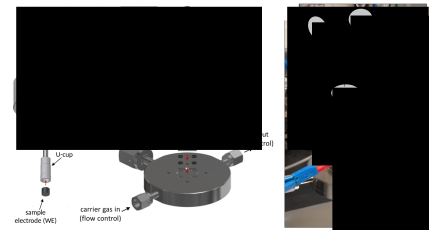
\includegraphics[width=\textwidth]{02_Tools/fig/chipECMS_diagrams_2.png}
	\caption{Diagrams of \textbf{(a)} the cell + working electrode assembly and \textbf{(b)} The cell + chip + interface block assembly. \textbf{(c)} Photo of the setup in use. From Paper \ref{Trimarco2018}}
	\label{fig:chipECMS2}
\end{figure}

The membrane chip is intended as a \textit{window} into what is happening on (or more specifically, what is desorbing from) the surface of an electrochemical sample. This requires setting up a three-electrode setup with the working electrode parallel to and close to the membrane. We accomplish this with an \textit{EC-MS cell}, diagrammed on the top-left of Figure \ref{fig:chipECMS}a and in Figure \ref{fig:chipECMS2}a. The cell is most simply described as a piece of polychlorotrifluoroethylene (PCTFE or Kel-F) with holes machined in it. The holes include a cavity through the center for the working electrode assembly. We use the Change-Disk RDE equipment commercially available from Pine Research Instruments for quick and versatile sample exchange. This system uses a PTFE U-cup, which is squeezed slightly between the sample and the cell, to hold the sample in place. The sample can be any 5 mm disk. The distance between the sample and the membrane of the chip, the \textit{working distance}, is defined by a Teflon spacer, and is 100 $\mu$m throughout this Thesis. The volume between the surface of the working electrode and the membrane chip is called the \textit{working volume}. The concentric 7 mm membrane and 5 mm membrane give rise to a 1 mm x 100 $\mu$m \textit{edge volume} which is bound by the membrane but not the working electrode. The high aspect ratio of this edge volume ensures that little to no analyte produced at the electrode is lost by lateral diffusion. 

The working volume is connected via channels in the EC-MS cell going from just past the edge volume to threaded openings at the top, which are generally fitted with Luer adapters for interfacing with liquid pathway components. In two of these, we place a piece of custom-made glassware with a Luer tip, a ceramic frit to prevent convection, and a large cylindrical volume above. These glassware house the reference and counter electrodes. The other two openings are then used as electrolyte inlet and outlet. The full assembly is shown in the photograph in Figure \ref{fig:chipECMS2}c. To avoid bubbles, the cell must be filled with electrolyte through the inlet before the reference and counter glassware are inserted.

As mentioned at the start of this chapter, chip EC-MS has two advantages over conventional systems for fundamental studies in electrocatalysis:

\begin{enumerate}
\item Extremely high sensitivity. This is possible because the chip membrane serves as an equilibration step, letting volatile gases evaporate without sucking in solvent. The very low solvent flux means that no differential pumping stage is necessary, unlike DEMS. Furthermore, the low solvent flux is the reason it is possible to run long experiments without flowing electrolyte. Together, this means that \textit{every molecule of volatile product produced on the electrode will make it to the mass spectrometer} 

\item The ability to quickly dose and purge reactant gases. This is possible because the equilibrium of the gas-liquid interface at the chip's membrane works both ways: dissolved gases are released, and the gas fed into the chip saturates the electrolyte in the working volume.
\end{enumerate}

Since electrolyte is not flowed during experiments, the cell is a a \textit{stagnant thin-layer} cell. The working volume functions as a perfect diffusion layer, making it relatively easy to model mass-transport in the system. This mass-transport model was first presented in my Master's Thesis\cite{Scott2016_MSc}, and later refined and verified experimentally in Paper \ref{Trimarco2018}. I will not redevelop the model here, but I will use its results from time to time throughout this Thesis.

\subsection{Chip EC-MS: implementation}\label{subsec:setups}

In practice, an external system for vacuum and gas handling is needed to realize the advantages of high sensitivity and quick reactant gas dosing and purging made possible by chip EC-MS. This Subsection describes two such vacuum systems that I worked on during this PhD project. The vast majority of my work was done on the so-called ``Sniffer setup'' at DTU. During my external stay in professor Zhenhai Wen's group at the Chinese Academy of Sciences (CAS) in Fuzhou, I designed a more compact version, which became the EC-MS 200A. A reader who is not interested in these practical details may wish to skip this Subsection. 

In the spirit of making this Thesis useful to my colleagues, Appendix \ref{app:instructions} describes procedures for changing chip and changing carrier gas for each of these setups with reference to the valve diagrams.

\vspace{1cm}
\textbf{\large The Sniffer Setup at DTU:}

\begin{figure}[h!]
	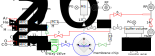
\includegraphics[width=\textwidth]{02_Tools/fig/setup_sniffer.png}
	\caption{Valve diagram of EC-MS setup at DTU. Adapted from Paper \ref{Trimarco2018}. Red: components installed since that publication. Green: The 6-way valve was removed since then as well as the pneumatic valves before the pressure controllers, which were re-purposed. Blue: The interface block, as well as the valve right before it, were replaced to minimize the intervening volume, enabling faster exchange of gases.}
	\label{fig:sniffer}
\end{figure}
Figure \ref{fig:sniffer} shows a valve diagram of the sniffer setup. Most of this setup was built during Daniel Trimarco's PhD project\cite{Trimarco2017_PhD}, and described in Paper \ref{Trimarco2018}. Colors indicate the parts that I have removed (green) or added (red) since Paper \ref{Trimarco2018}'s publication.

On the left of the diagram are mass flow controllers (MFC's) which can be used to switch between up to four gases at time. Switching between gases sharing an MFC, f.eks. Ar and He, requires pumping down behind the MFC through a line not shown. Moving right, we refer to the volume between Valves 7, 8, 9, 10, 11, and 12 and PC 1 as the \textit{gas manifold}. The gas manifold can be evacuated through Valve 7 and filled up from one of the MFC's while regulating the pressure with a pressure controller (PC), PC1.

Carrier gas from the gas manifold enters the interface block via Valve 8. The interface block guides it through the carrier gas reservoir channel of the chip, from which it fills the chip's sampling volume and saturates the electrochemical environment. Fast carrier gas exchange thus requires that the volume between valve 8 and the chip, the \textit{carrier gas inlet volume} is as small as possible. This is because the carrier gas inlet volume, unlike the gas manifold, cannot be pumped down, as the resulting vacuum in the sampling volume of the chip would suck in electrolyte. The design of the carrier gas inlet volume can also be optimized with regards to flow patterns to minimize mixing of the old and new carrier gas. 

We refer to the volume between PC1, PC2, and Valves 1, 5, 6, and 7 as the \textit{pumping manifold}. There are actually three possible ways to pump on the pumping manifold: (1) Directly to the \textit{roughing pump} (RP) through Valve 6, or (2-3) through a buffer volume and then a \textit{turbo molecular pump} (TMP or just turbo pump) via either a (2) valve 2 and a needle valve or (3) a gate valve. 
%Of these options, the direct roughing pump connection is the only one that can quickly remove a large amount of gas, as this would damage the turbo pump. Valve 14 should be closed while gas is fed directly to the roughing pump, as the pressure behind the turbo pump must also be kept low during operation. On the other hand, the turbo pump is required to reach high vacuum, which it can do slowly for a moderate amount of gas through the needle valve or quickly for a small amount of gas through the gate valve.

During operation, carrier gas is flowing from the gas manifold to the pumping manifold through the chip, and its pressure is regulated by PC2, which is set to 1 bar for all of the experiments in this Thesis. Excess carrier gas flows through PC2 to the pumping manifold where it is ultimately removed through the roughing pump, typically via the buffer volume and needle valve, so that valve 14 can remain open.

When a new chip is installed, the \textit{post-capillary volume} bound by the chip, Valve 13, and Valve 5 is vented to atmospheric pressure, and must be pumped down to high vacuum before connecting the experiment to the mass spectrometer. The mass spectrometer is always held at high vacuum by its own designated turbo and roughing pumps. The mass spectrometer of the sniffer setup is a Pfeiffer QMA125.

The procedures for chip pump-down and carrier gas exchange are described in Appendix \ref{app:sniffer}.

\vspace{1cm}
\textbf{\large The ECMS-200A in Fuzhou:}

\begin{figure}[h!]
	\centering
	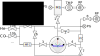
\includegraphics[width=0.75\textwidth]{02_Tools/fig/setup_Fuzhou.png}
	\caption{Valve diagram of EC-MS setup at Fuzhou. In reality, at the time of writing this thesis, the pressure controller is actually a modified pressure regulator, which works but is not as stable.}
	\label{fig:Fuzhou}
\end{figure}

The sniffer setup described above can be considered a ``delux setup'' with an excess of components to maximize functionality. The group in Fuzhou asked me to design a ``budget setup'' which captured the central advantages of chip EC-MS with as few components as possible. They then built my design, shown in Figure \ref{fig:Fuzhou} with the outside help from a Chinese mass spectrometer company, Quantang Instruments. Much to my frustruation, Quantang built a box around the valve system, making it quite tedious to make changes to the system, and put their logo and the name ECMS200A on the box.

All of the concepts are the same as for the sniffer setup, but the operation is different. The procedures for chip pump-down and carrier gas exchange are described in Appendix \ref{app:Fuzhou}. The cost of having one less Turbo pump is the need to wait for long pumping periods and to turn off the filament of the mass spectrometer when changing chips. The carrier gas exchange procedure is actually slightly simpler than that of the sniffer setup and saves three MFC's and a PC. The only disadvantage is that, with only one MFC, it is not easy to prepare a controlled gas mixture (a functionality I have rarely used on the sniffer setup).

\vspace{1cm}
\textbf{\large Spectro Inlets:}

\begin{figure}[h!]
	\centering
	\includegraphics[width=0.75\textwidth]{02_Tools/fig/spectro.png}
	\caption{Photos of the setup at Spectro Inlets ApS. From their website: \url{https://spectroinlets.com/}}
	\label{fig:spectro}
\end{figure}
Finally, I should mention that there is now a commercially available setup which combines the best of both worlds: The functionality of the Sniffer setup and the simplicity and compactness of the ECMS200A. This is made possible in part due to some custom vacuum components. The setup, sold by Spectro Inlets ApS, is shown in the photographs in Figure \ref{fig:spectro}. I have been involved in conversations aiding the development of this setup, as a kind of test user, but can't go to detail here on its design. The Spectro Inlets setup also comes with a software automating the chip pump-down and carrier gas exchange procedures. The procedures described in Appendix \ref{app:instructions} for the other two setups are thus simplified to pressing a button.


\subsection{Example experiments: RHE potential measurement and CO stripping}\label{subsec:examples}
Here I show two examples of common electrochemistry experiments as seen through the window of chip EC-MS. These two experiments also demonstrate the utility of the gas-exchange functionality, and happen to be quite interesting when instead done in isotope-labeled electrolyte. Isotope-labeled versions of these two experiments are shown later in this Chapter, in Subsections \ref{subsec:isotope_RHE} and \ref{subsec:isotope_CO2}.

The first experiment is a measurement of the reference electrode potential on the reversible hydrogen electrode (RHE) scale. The reversible hydrogen electrode potential is defined as the potential at which the hydrogen evolution and hydrogen oxidation reactions (HER and HOR, respectively) are at equilibrium in electrolyte saturated by 1 bar hydrogen:
\begin{equation}
\ch{2 (H+ + e- ) <-> H2} \label{rxn:HER2p1}
\end{equation}
This situation can be easily created in a chip EC-MS setup using hydrogen as the carrier gas and a platinum electrode as the sample, since platinum is an excellent catalyst for the HER/HOR\cite{Nørskov2005a, Kemppainen2015, Tymoczko2016}. 

\begin{figure}[h!]
	\centering
	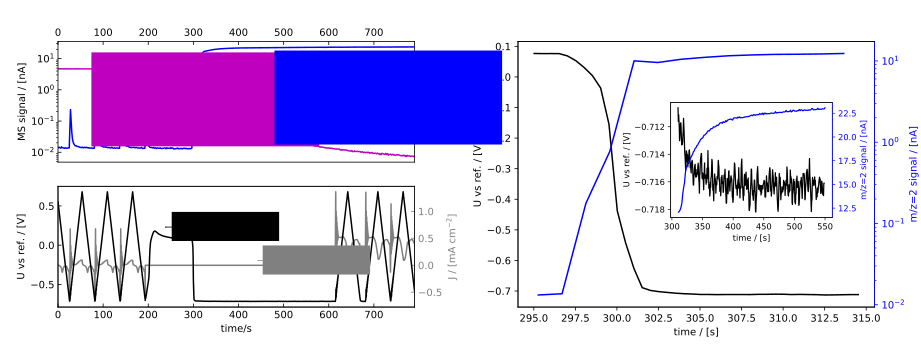
\includegraphics[width=\textwidth]{02_Tools/fig/RHE_calibration.png}
	\caption{RHE calibration experiment using a polycrystalline platinum electrode in 0.1 M \ch{HClO4}. \textbf{(a)} EC-MS plot with mass spectrometer signals in the top panel and the concurrent electrochemical data in the lower panel. \textbf{(b)} A zoom-in on the time at which the carrier gas is switched from helium to hydrogen while the electrode is at OCP, showing the electrode potential (black, left y-axis) co-plotted with the m/z=2 signal (blue, right y-axis)}.
	\label{fig:RHE_cal}
\end{figure}

The experiment is shown in  in Figure \ref{fig:RHE_cal}a as an \textit{EC-MS plot}, in which the electrochemical potential (left y-axis) and current (right y-axis) are plotted against time in the bottom panel and the concurrent mass spectrometry data is shown in the top panel on the same time axis.
\footnote{Customized EC-MS plots, including all of the ones presented in this Thesis, can be produced in one line of code with the highly versatile \texttt{plot\_experiment} function of the \ch{EC\_MS} python package, described in Appendix \ref{app:EC_MS}.}

Starting from the left: the platinum electrode is cycled between -0.7 and +0.7 V vs the reference electrode (Hg/\ch{HgSO4}) in helium-saturated electrolyte. Three full cycles are shown. Hydrogen is produced near the cathodic potential limit, giving rise to an increase in the mass spectrometer signal at m/z=2. The electrode is set to open-circuit potential (i.e., the current is set to zero) at the cathodic potential limit of the fourth cycle. This results in less \ch{H2} than the first cycles, since in the first cycles HER continues at the start of the anodic scan. The open-circuit potential then drifts in the anodic direction until just before the onset of \ch{$*$ OH} adsorption, which would draw current. At 300 s, \ch{H2} is flowed through the chip, replacing \ch{He} in the carrier gas reservoir channel. The \ch{H2} very quickly enters the sampling volume of the chip, giving rise to a m/z=2 signal in the mass spectrometer. Simultaneously, the \ch{H2} saturates the electrolyte in the working volume. The first \ch{H2} molecules to encounter the electrode are immediately oxidized to \ch{H2O} because there is a substantial overpotential to drive the HOR (Reaction \ref{rxn:HER2p1} in the leftwards direction). However, since the electrode is at OCP, there is nowhere for the resulting electrons to go, and so they change the charge density of the electrochemical double layer, which functions as a capacitor\cite{Chan2015a}. This causes the potential to drop very quickly. The electrode soon reaches a potential at which Reaction \ref{rxn:HER2p1} is in equilibrium. This equilibrium potential depends on the partial pressure of \ch{H2}, and so the potential continues to change slowly as \ch{H2} fully replaces \ch{He}. 

The example in Figure \ref{fig:RHE_cal} is unfortunately not the most elegant gas exchange, as indicated by the inflection points in the MS signals as \ch{H2} replaces \ch{He} in Figure \ref{fig:RHE_cal}a. (This results from an overpressure in the gas manifold before opening Valve 8 in Figure \ref{fig:sniffer}, which causes turbulence and gas mixing in the carrier gas inlet volume.) Figure \ref{fig:RHE_cal}b shows the simultaneous change in the \ch{H2} signal and electrode potential during the gas switch. The electrode potential becomes stable to within a few millivolts just 10 seconds after the switch, but the last $\approx$ 2 mV to the RHE potential of -0.717 V vs the reference electrode take about 100 s (inset). This is, nonetheless, a much faster RHE measurement than can be accomplished when a macroscopic amount of electrolyte, for example in an H cell, needs to be fully purged with hydrogen. Such RHE measurements are used routinely to calibrate the reference electrode potential on the RHE scale in a new electrolyte.

\begin{figure}[h!]
	\centering
	\includegraphics[width=\textwidth]{02_Tools/fig/Trimarco2018_fig03.png}
	\caption{Experiments showing HER, OER, CO oxidation, and CO stripping on Pt in 1.0 M \ch{HClO4}.  \textbf{(a)} and \textbf{(c)} show EC-MS plots and \textbf{(b)} and \textbf{(d)} each show two parts of the respective data set co-plotted against potential. \ch{He}, \ch{CO}, \ch{H2}, \ch{O2}, and \ch{CO2} fluxes were obtained by calibrating the m/z=4, 28, 2, 32, and 44 signals, respectively, according to the procedures described in Section \ref{sec:quantification}. For a detailed discussion, see Paper \ref{Trimarco2018}.}
	\label{fig:fig3}
\end{figure}

Figure \ref{fig:fig3}, from Paper \ref{Trimarco2018}, demonstrates platinum electrochemistry involving carbon monoxide (CO). Here, the potential has been calibrated to the RHE scale as described above, and the mass spectrometer signals have been calibrated as described in Section \ref{sec:quantification}. Figure \ref{fig:fig3}a shows a long electrochemistry program including constant-potential steps and cyclic voltammatry, and a switch from He to CO in the middle. It is described in detail in the paper. Two cycles from this program (one in He and one in CO) are selected and plotted vs potential in Figure \ref{fig:fig3}b, as is popular among users of DEMS and OLEMS.

Figure \ref{fig:fig3}c and d show a CO stripping experiment, a common method of characterizing noble metal surfaces in electrocatalysis\cite{Mayrhofer2005, Koper2009, Ganassin2017, Jensen2017_PhD}. It consists of two steps: adsorption of CO, and oxidation of adsorbed CO, given in Reactions \ref{rxn:COads} and \ref{rxn:COstrip}, respectively:
\begin{align}
\ch{CO + $*$ &-> $*$ CO}\label{rxn:COads}\\
\ch{$*$ CO + H2O &-> $*$ + CO2 + 2 (H+ + e- )}\label{rxn:COstrip}
\end{align}
To study the oxidation of surface-adsorbed *CO in isolation, the *CO dosed in the first step has to be purged from the electrolyte before the second step.

In Figure \ref{fig:fig3}c, after an initial cyclic voltammagram, a short pulse of CO is dosed using the 6-way valve in Figure \ref{fig:sniffer} and adsorbs on the surface, as indicated by the CO displacement current at $\approx$190 s. After the CO dose, the first cycle shows no \ch{H2} signal or hydrogen adsorption current (Figure \ref{fig:fig3}d), indicating the surface is fully poisoned by adsorbed CO. The anodic scan shows a CO stripping current starting at $\approx$0.7 V vs RHE. The final cycle is identical to the cycle before the \ch{CO} dose. We like to brag that this is the fastest complete CO stripping experiment ever reported in the literature.

This experiment also demonstrates the sensitivity of the system: the integrated \ch{CO2} signal corresponds to approximately 0.75 ML, i.e. 3 CO molecules adsorbed for every 4 Pt surface atoms; and the integrated \ch{H2} signal at 410 s corresponds to approximately 0.05 ML.

\subsection{Disadvantages}\label{subsec:disadvantages}

The attentive reader might be wondering why the shapes of the \ch{CO2} and \ch{H2} signals in Figure \ref{fig:fig3}c are so different. Whereas the \ch{H2} signal peaks at 10 pmol/s within a second or two of the cathodic potential limit and has completely passed a few seconds after that, the \ch{CO2} signal, which corresponds to $\approx$ 15 times as many molecules, also peaks at $\approx$ 10 pmol/s but then falls very slowly. This is especially annoying when data are plotted against potential (Figure \ref{fig:fig3}d), because the tail of the \ch{CO2} signal lasts well into the cathodic scan, even though all of the \ch{CO2} is produced by the electrode surface during the anodic scan. Since the ability to detect a signal is described by its height as well as its area, chip EC-MS is in effect less sensitive to \ch{CO2} than \ch{H2}.

It turns out that this is an inevitable part of chip EC-MS, inseparable from its major advantage of low solvent evaporation\cite{Scott2016_MSc}. Both are cases of a general fact: the characteristic time for an analyte to leave the working volume and enter the mass spectrometer is strongly dependent on its Henry's-Law constant of volatility. This is defined as the equilibrium ratio of its partial pressure in the gas phase to its concentration in the aqueous phase:
\begin{equation}
K_H^i = \frac{p^i}{c^i}
\end{equation}
Because there is equilibrium across the chip membrane, the partial pressure of a uniformly dissolved analyte in the chip's sampling volume, and thus the rate at which it is removed through the chip capillary, is proportional to its Henry's-Law constant. The characteristic time, taking both diffusion through the working volume and evaporation across the chip's membrane, for removal of analyte $i$ from the working volume is\cite{Scott2016_MSc}:
\begin{equation}
\tau^i = \frac{L^2}{2D^i} + \frac{L p^0_\text{chip}A_\text{el}}{\dot{n}^0_\text{cap} K^i_H}
\end{equation}
where $L$ is the working distance, $D^i$ is $i$'s diffusion constant in water, $p^0_\text{chip}=1$ bar is the total pressure in the chip, and $\dot{n}^0_\text{cap}$ is the combined flux through the capillary. For all but the least soluble gases (including \ch{H2} and \ch{O2}), this is dominated by the second term, which can vary many orders of magnitude. Thus, while any analyte with any vapor pressure will in principle reach the mass spectrometer eventually, detection of liquid products is highly unpractical. The characteristic time is (ref. \cite{Scott2016_MSc} and Paper \ref{Trimarco2018}) 2 s for \ch{H2}, 3 s for \ch{O2}, 27 s for \ch{CO2}, and $2.5\cdot10^{5}$ s for ethanol.

The question then comes up:
\begin{question}
	With respect to the sensitivity of product detection, when is it advantageous to use chip EC-MS and when is it advantageous to use conventional DEMS?
\end{question}
\begin{figure}[h!]
	\includegraphics[width=\textwidth]{02_Tools/fig/fig07_old.png}
	\caption{Model comparing the sensitivity of chip EC-MS to conventional DEMS via the collection efficiency in a hypothetical flow setup. Adapted from Paper \ref{Trimarco2018}.}
	\label{fig:sensitivity}
\end{figure}
Figure \ref{fig:sensitivity} rephrases this question in terms of \textit{collection efficiency} in a hypothetical flow setup: if an analyte dissolved in an electrolyte is flowing past the vacuum inlet (essentially the collection chamber in a dual thin-layer flow cell\cite{Jusys1999, Clark2015}), will more molecules of the analyte reach the mass spectrometer if the inlet is chip EC-MS or DEMS? To answer this question, I modified the stagnant thin-layer mass transport model to give the concentration profile in such a flowing collection volume\cite{Scott2016_MSc}. The model is diagramed in Figure \ref{fig:sensitivity}a and three cases are shown in Figure \ref{fig:sensitivity}c-d. The resulting collection efficiencies are plotted as a function of Henry's-law constant in Figure \ref{fig:sensitivity}b. For light gases like \ch{H2}, chip EC-MS wins due to the lack of a differential pumping stage. For volatile liquids like ethanol, DEMS wins because the much faster non-equilibrium mass transport of products into the first stage of the vacuum chamber outweighs the loss due to differential pumping. 

Thus, chip EC-MS is not ideal for, e.g., \textit{in-operando} studies of \ch{CO2} reduction, in which production rates can be high but the interesting products are liquid at room temperature.

\vspace{5mm}
Furthermore, while the sensitivity and ability to quickly dose reactant gases are major advantages for chip EC-MS in fundamental studies, it should not be considered a full substitute for a rotating disk electrode (RDE) setup or other setup optimized for cyclic voltammatry. It can sometimes be challenging to get good cyclic voltammagrams in the setup. Figure \ref{fig:current_distribution}a shows electrochemistry data from Figure \ref{fig:RHE_cal}a plotted against potential. The magenta cycle is with He as the carrier gas, and the blue cycle is with \ch{H2} as the carrier gas. The \ch{H2} CV is shifted up with respect to the \ch{He} CV due to a mass-transport-limited hydrogen oxidation current until the platinum surface starts to oxidize at 0.9 V vs RHE and becomes less active for hydrogen oxidation. This all makes sense, but the CV's are dominated by an artifact in the start of the anodic scan: rapid oscilations of current and potential. 

\begin{figure}[h!]
	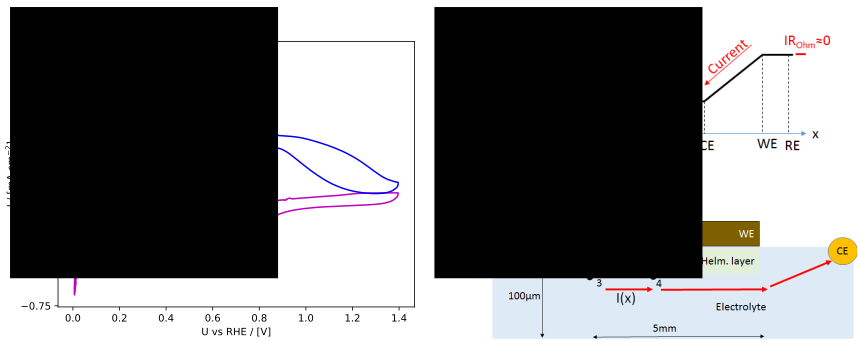
\includegraphics[width=\textwidth]{02_Tools/fig/nonideal_current_distribution.png}
	\caption{\textbf{(a)} CV's in He (magenta) and \ch{H2} from Figure \ref{fig:RHE_cal}. The squiggles are the result of oscillations caused, in part, by electrolytic resistance accross the surface of the sample. \textbf{(b)} Schematic diagrams of electrode connections to the working volume, indicating that while the conventional ohmic resistance is zero, the resistance within the working volume means that the electrochemical potential is not uniform; adapted from my Master's Thesis\cite{Scott2016_MSc}}.
	\label{fig:current_distribution}
\end{figure}

These oscillations are worse the less conductive the electrolyte is, and occur most often when there is a sudden change in absolute current density, such as (in this case) right at the scan polarity change in the hydrogen region. The oscillations are attributed to the challenge of controlling the potential when there is a large resistance through the electrolyte from one end of the electrode to the other, first described for this setup in my Master's Thesis\cite{Scott2016_MSc}. 

Briefly, the conventional ohmic drop in the EC-MS cell is zero, since the current through the electrolyte is conducted between the working electrode (WE) and the counter electrode (CE), but potential is measured to the reference electrode (RE) on the opposite side of the working electrode (top half of Figure \ref{fig:current_distribution}b. Indeed, potential electrochemical impedance spectrometry (PEIS) measurements in the sniffer setup show a vertical line through zero resistance on the real axis. This is despite the fact that there are large resistances in the cell, most notably in the working volume itself. This resistance can lead to the potential drop across the Helmholtz layer on two parts of the working electrode not being identical, as indicated in the bottom of Figure \ref{fig:current_distribution}. How exactly this leads to oscillations, I do not fully understand.

I realized remarkably late in my PhD project that setting the bandwidth on the Biologic SP-150 Potentiostat to 3, with everything else set up perfectly, could usually remove this artifact. Before that, I had realized that putting a 100 Ohm resistor behind the working electrode helps. This effectively introduces a conventional ohmic resistance, which seems to help the potentiostat avoid such oscillations, and is easy to correct for afterwards when plotting CV's.

The maximum size of the difference in electrochemical potential across the working electrode is important to know, as it is a possible source of error in activity measurements, such as those that will be presented in Section \ref{sec:low_O2}. For 0.1 M \ch{HClO4} (the electrolyte used in that Section), the resistance from one end of the working volume to the other is on the order of
\begin{equation}
R = \frac{1}{\kappa}\frac{d}{L\frac{d}{2}} = \frac{2}{\kappa L} = \frac{2}{4.2 \left[\frac{\text{S}}{\text{m}}\right]\cdot 100[\mu\text{m}]} = 4.8 [\text{k}\Omega]
\end{equation}
Where $\kappa$ is the conductivity of the electrolyte, $L$ is the working distance, $d$ is the diameter of the disk, and to make sure the resistance is overestimated I've approximated the geometry as a resistor with a cross section of $L\cdot\, d/2$ but a length of $d$. 

This is a huge resistance! The maximum current densities used in this thesis are approximately 100 $\mu$A (0.5 mA/cm$^2$ geometric current density). At this current density, if we assume the worst case, that all of the current comes from the end of the working electrode closest to the reference electrode, then the potential at the end of the working electrode closest to the counter electrode could be off by as much as $100[\mu\text{A}]\cdot4.8 [\text{k}\Omega] = 0.48[\text{V}]$. The error is in the direction to \textit{increase the overpotential} of the current-drawing reaction on the part of the electrode close to the CE compared to what it should be according to the potential difference between WE and RE. This is a huge potential error! 

We are partially saved by two facts:
\begin{itemize}
	\item The worst case scenario is very far from the truth. In reality, there will be more current from the side of the working electrode closest to the counter electrode. In other words, an uneven current distribution will seek to alleviate an uneven potential distribution, not exacerbate it.
	
	\item The error is reduced at small current densities, which are the interesting ones for chip EC-MS anyway. In the same electrolyte at 1 $\mu$A (corresponding to 10 pmol/s of electrons), the error is less than a worst-case scenario of 4.8 mV difference, still not great but more acceptable.
\end{itemize}

Nonetheless, solving this should be a high priority for continued development of chip EC-MS. A promising solution is to fabricate chips with liquid through-holes, so that a counter electrode can be placed behind the chip and parallel to the working electrode. A first attempt at this is described in the Master's Thesis of Jesper Pan\cite{Pan2018_MSc}, and a second attempt is being led by Thomas Pedersen of DanChip.

To improve the mood after this discussion of problems with chip EC-MS, the next Section will focus on a positive aspect: the fact that 100\% of gaseous electrochemical products make it to the mass spectrometer makes chip EC-MS an excellent platform for \textit{absolute quantification} in mass spectrometry.